\documentclass[../../main]{subfiles}

\renewcommand\thesection{\arabic{section}}


\begin{document}

\section{Modern Day's Microcontrollers} \label{sec:}

That ``Ok Google'' model was develop around 10 years ago, and utilized
those day's DSPs. Let's see some of our day's popular microcontrollers.

\subsection{ESP32}

\begin{center}
    \renewcommand\arraystretch{2.0}
    \begin{tabularx} {\textwidth} {
            >{\raggedright \arraybackslash}X
            >{\centering \arraybackslash}m{6cm}
        }

        \toprule

        \vspace{0.5cm}
        Flash Memory: 4 MB
        &

        \multirow{3}{*}{
            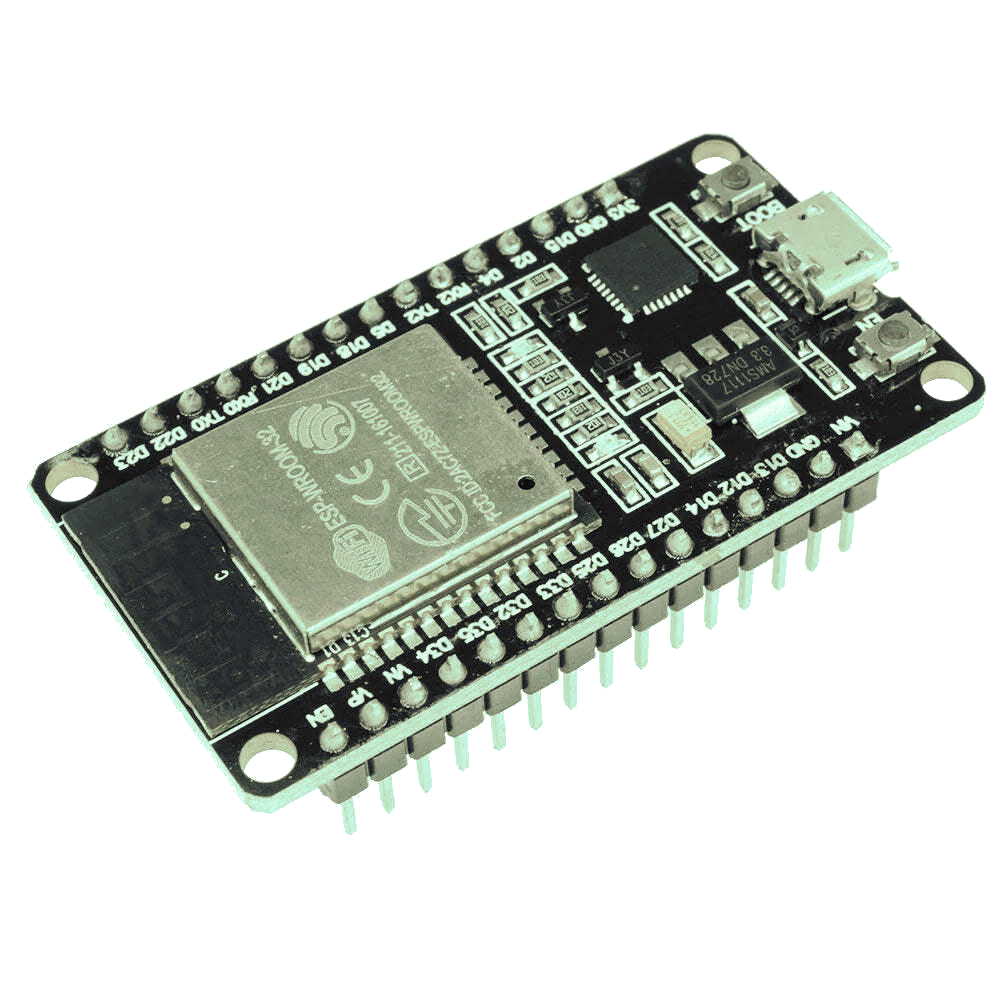
\includegraphics[
                trim = {0cm 1cm 0cm 0.2cm},
                width = 0.3\textwidth,
                clip,
            ]{pics/esp.png}
        }

        \\ \cmidrule{1-1}

        CPU Clock Speed: 240 MHz
        &

        \\ \cmidrule{1-1}

        RAM Available: 520 KB
        \vspace{0.5cm}
        &

        \\

        \bottomrule

    \end{tabularx}

    \captionof{table}{Table showcasing some of the specifications of ESP32.}
    \label{tbl:}

\end{center}

\subsection{Arduino UNO}

\begin{center}
    \renewcommand\arraystretch{2.0}
    \begin{tabularx} {\textwidth} {
            >{\raggedright \arraybackslash}X
            >{\centering \arraybackslash}m{6cm}
        }

        \toprule

        \vspace{0.5cm}
        Flash Memory: 32 KB
        &

        \multirow{3}{*}{
            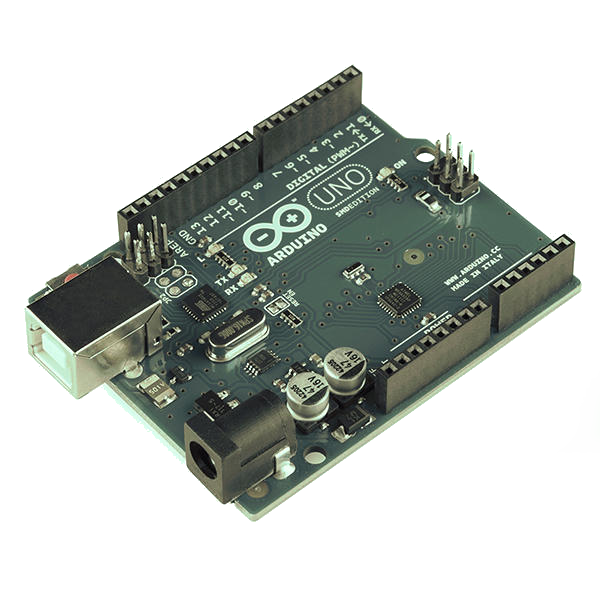
\includegraphics[
                trim = {0cm 0.5cm 0cm 0.2cm},
                width = 0.3\textwidth,
                clip,
            ]{pics/arduino.png}
        }

        \\ \cmidrule{1-1}

        CPU Clock Speed: 16 MHz
        &

        \\ \cmidrule{1-1}

        RAM Available: 2 KB
        \vspace{0.5cm}
        &

        \\

        \bottomrule

    \end{tabularx}

    \captionof{table}{Table showcasing some of the specifications of Arduino UNO.}
    \label{tbl:}

\end{center}

\subsection{Raspberry Pi Pico}

\begin{center}
    \renewcommand\arraystretch{2.0}
    \begin{tabularx} {\textwidth} {
            >{\raggedright \arraybackslash}X
            >{\centering \arraybackslash}m{6cm}
        }

        \toprule

        \vspace{0.5cm}
        Flash Memory: 2 MB
        &

        \multirow{3}{*}{
            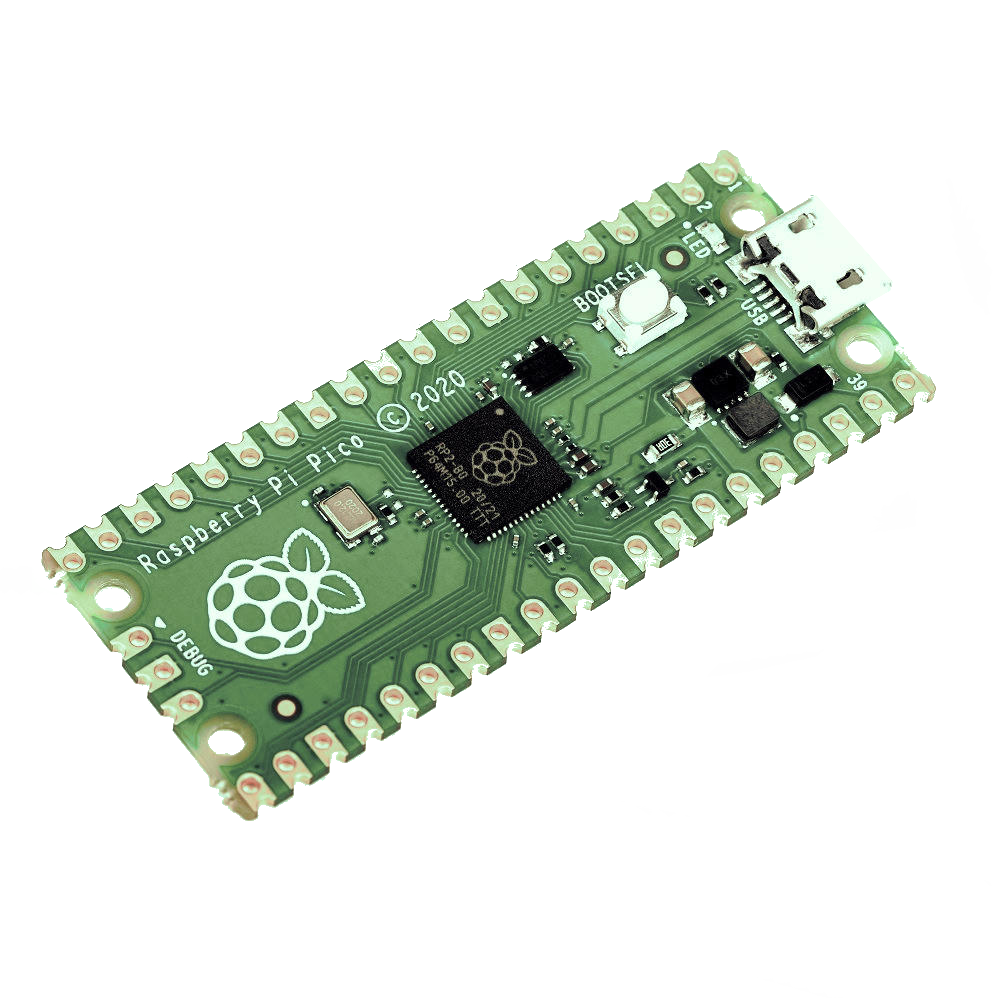
\includegraphics[
                trim = {0cm 1cm 0cm 0.2cm},
                width = 0.3\textwidth,
                clip,
            ]{pics/pico.png}
        }

        \\ \cmidrule{1-1}

        CPU Clock Speed: 125 MHz
        &

        \\ \cmidrule{1-1}

        RAM Available: 264 KB
        \vspace{0.5cm}
        &

        \\

        \bottomrule

    \end{tabularx}

    \captionof{table}{Table showcasing some of the specifications of Raspberry Pi Pico.}
    \label{tbl:}

\end{center}

\end{document}
